\section{Results}
This section presents findings from the user study evaluating LLM-adapted POI descriptions against manual baselines. Responses are summarized across three core metrics: significance, trustworthiness, and clarity. Comparative preference results and overall feedback are then reported.

Across 51 participants and 10 POIs, the study collected $N = 510$ ratings per condition for each metric (manual versus AI). Table~\ref{tab:metrics-summary} summarizes the distribution of ratings aggregated across all evaluations.

\begin{table}[h]
  \centering
  \small
  \begin{tabular}{@{}lcccccc@{}}
    \toprule
    & \multicolumn{2}{c}{\textbf{Significance}} & \multicolumn{2}{c}{\textbf{Trust}} & \multicolumn{2}{c}{\textbf{Clarity}} \\
    \cmidrule(lr){2-3} \cmidrule(lr){4-5} \cmidrule(lr){6-7}
    \textbf{Level} & Man. & AI & Man. & AI & Man. & AI \\
    \midrule
    1--2 (Low)  & 5.5  & 6.3  & 10.0 & 7.3  & 7.1  & 5.7 \\
    3 (Neutral) & 27.1 & 23.1 & 33.3 & 27.4 & 28.8 & 21.4 \\
    4--5 (High) & 67.4 & 70.6 & 56.7 & 65.3 & 64.1 & 72.9 \\
    \bottomrule
  \end{tabular}
  \vspace{0.9em}
  \caption{Distribution of User Ratings (\%) for Manual vs.\ AI Descriptions ($N=510$)}
  \label{tab:metrics-summary}
\end{table}

% Full count tables are available in the accompanying research report.

\subsection{Perceived Significance}
Participants rated both description versions on how effectively they communicated the significance and offerings of each POI using a 5-point Likert scale ranging from Strongly Disagree to Strongly Agree. Figure~\ref{fig:significance} illustrates the distribution of responses for manual and AI-generated descriptions.

\begin{figure}[h]
  \centering
  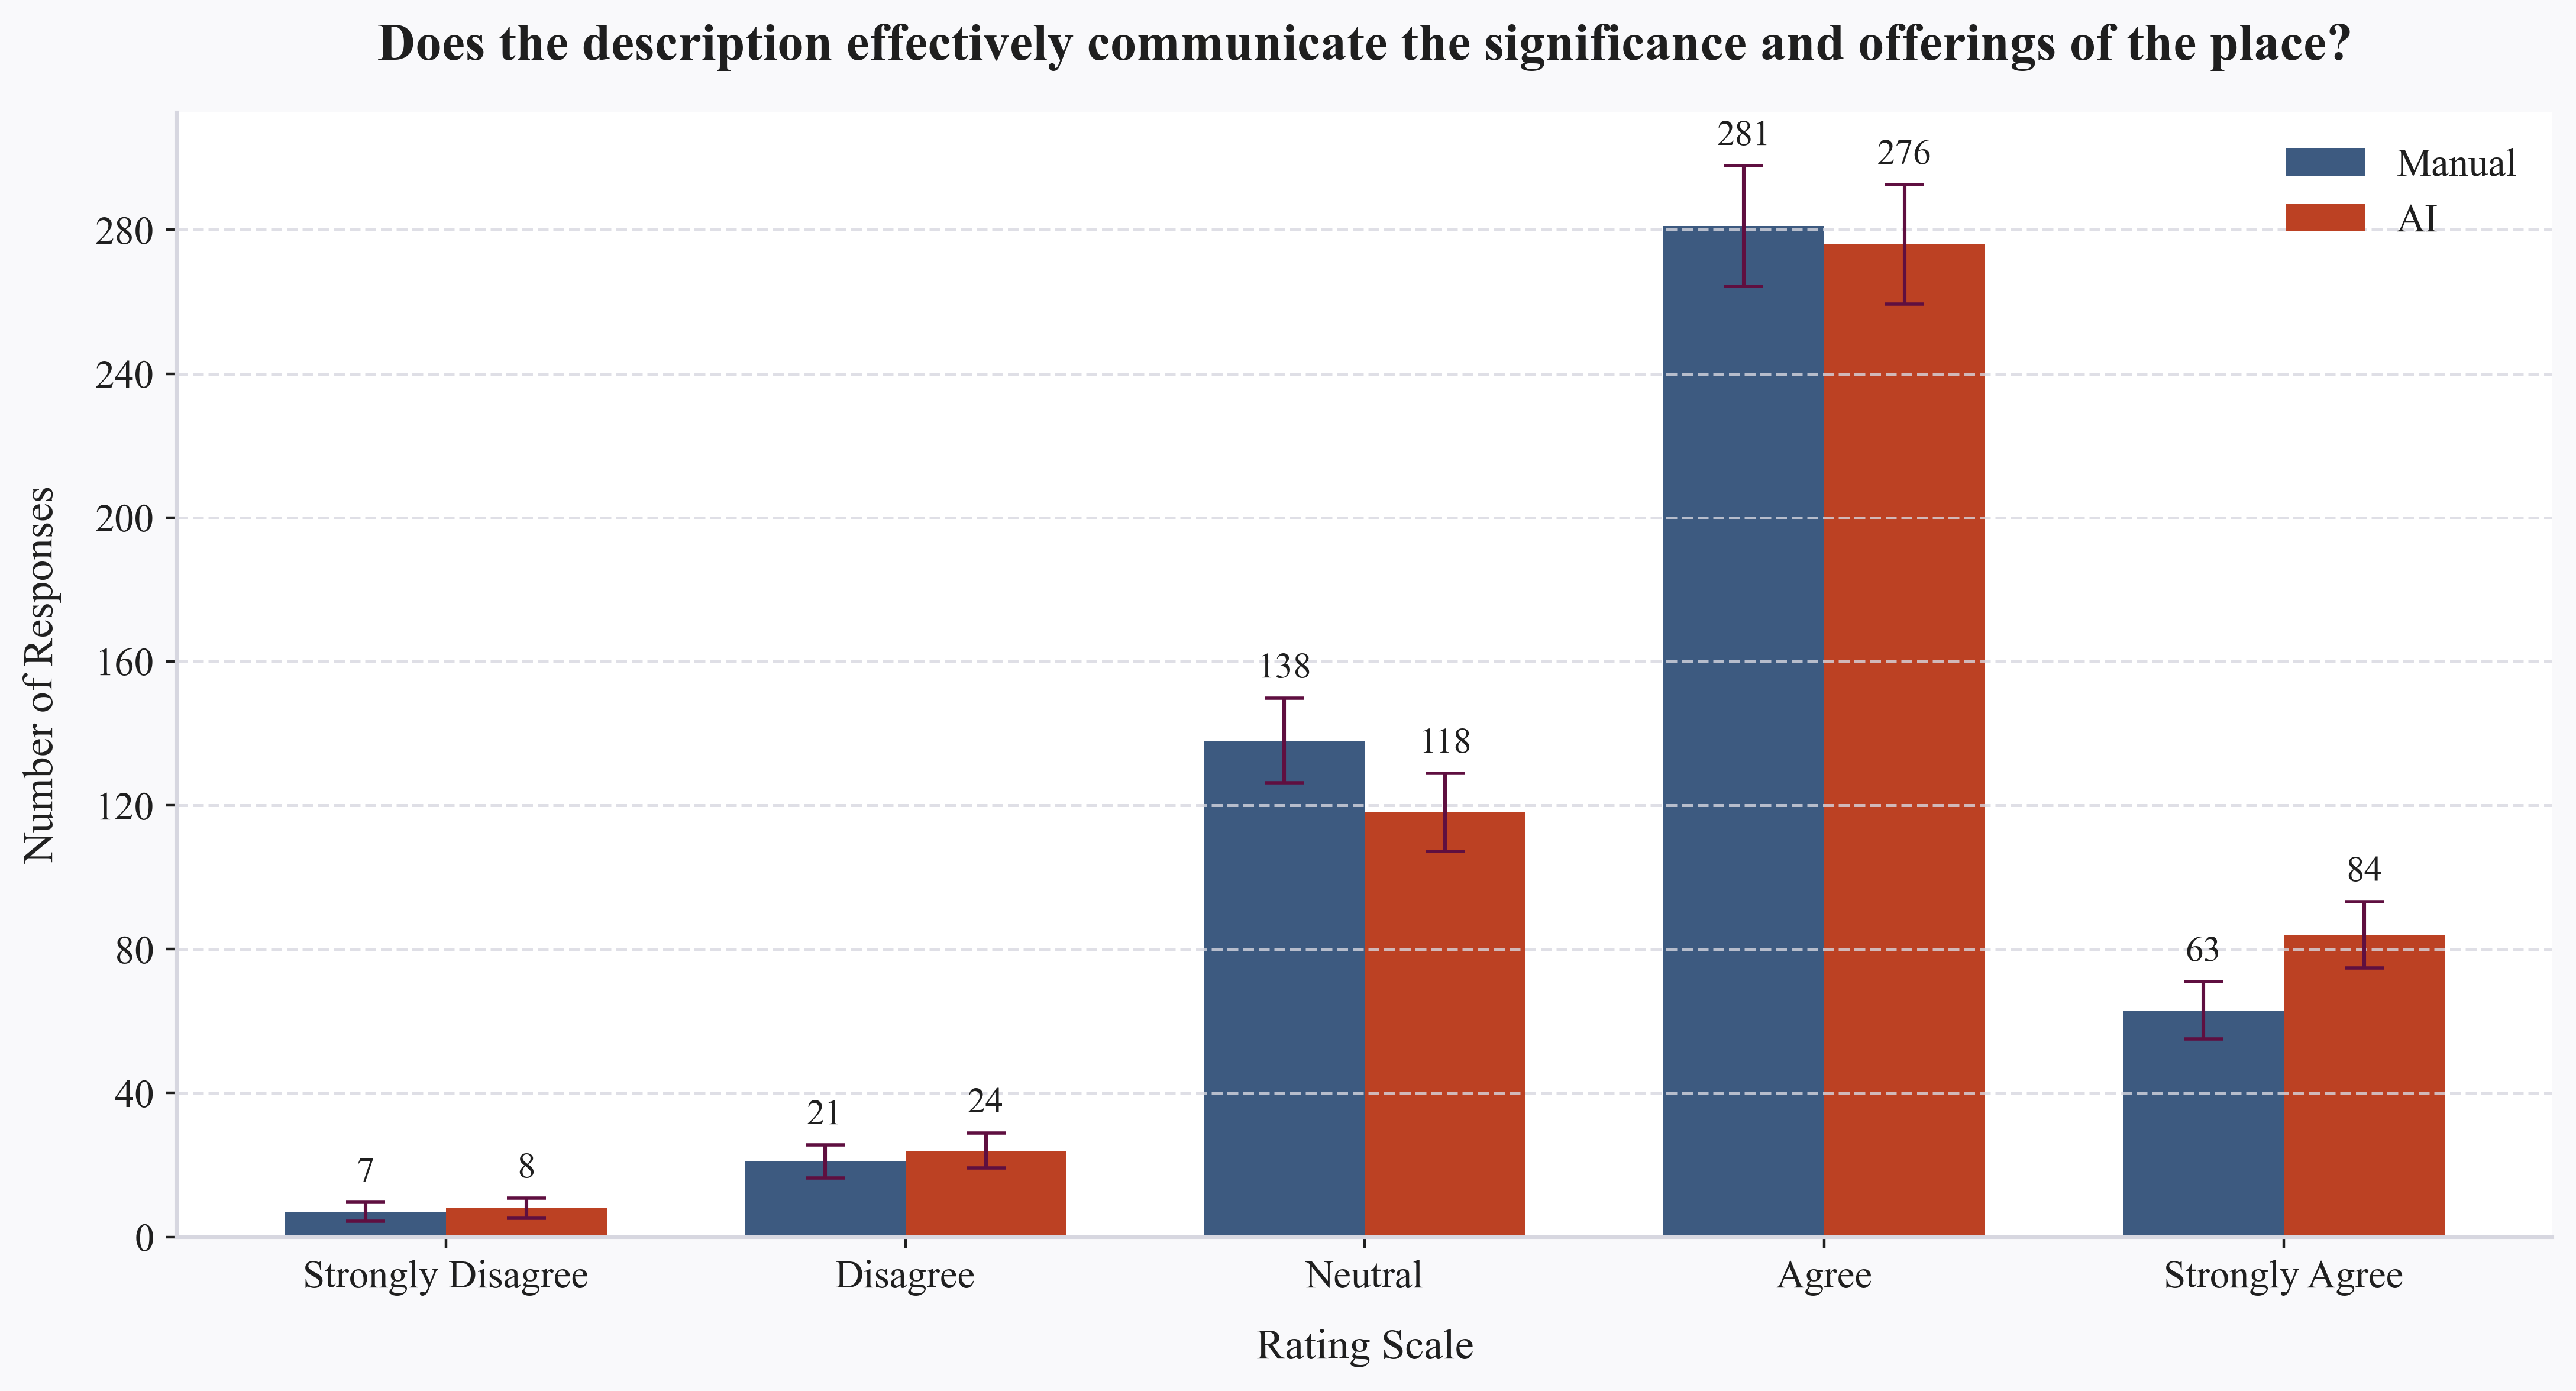
\includegraphics[width=0.85\linewidth]{figures/significance_comparison.png}
  \caption{Comparison of perceived significance between manual and AI-generated descriptions. Error bars represent Poisson-style standard error estimates computed on raw counts ($\sqrt{n}$).}
  \Description{Bar chart comparing manual and AI description ratings for significance communication}
  \label{fig:significance}
\end{figure}

Both description types received predominantly positive ratings (Table~\ref{tab:metrics-summary}). AI-generated descriptions shifted responses away from neutral toward stronger endorsement (e.g., Strongly Agree increased from 63 to 84 ratings). However, the pooled chi-square test did not indicate a statistically reliable difference in the overall distribution ($\chi^2(4) = 4.87$, $p = 0.3005$). The corresponding effect size was small (Cramer's $V = 0.069$, computed with $N=1020$ pooled observations), suggesting similar perceived significance between conditions.

\subsection{Trustworthiness}
Trustworthiness was assessed on a 5-point scale ranging from Not at all to Extremely. Figure~\ref{fig:trust} presents the comparative distribution of trust ratings.

\begin{figure}[h]
  \centering
  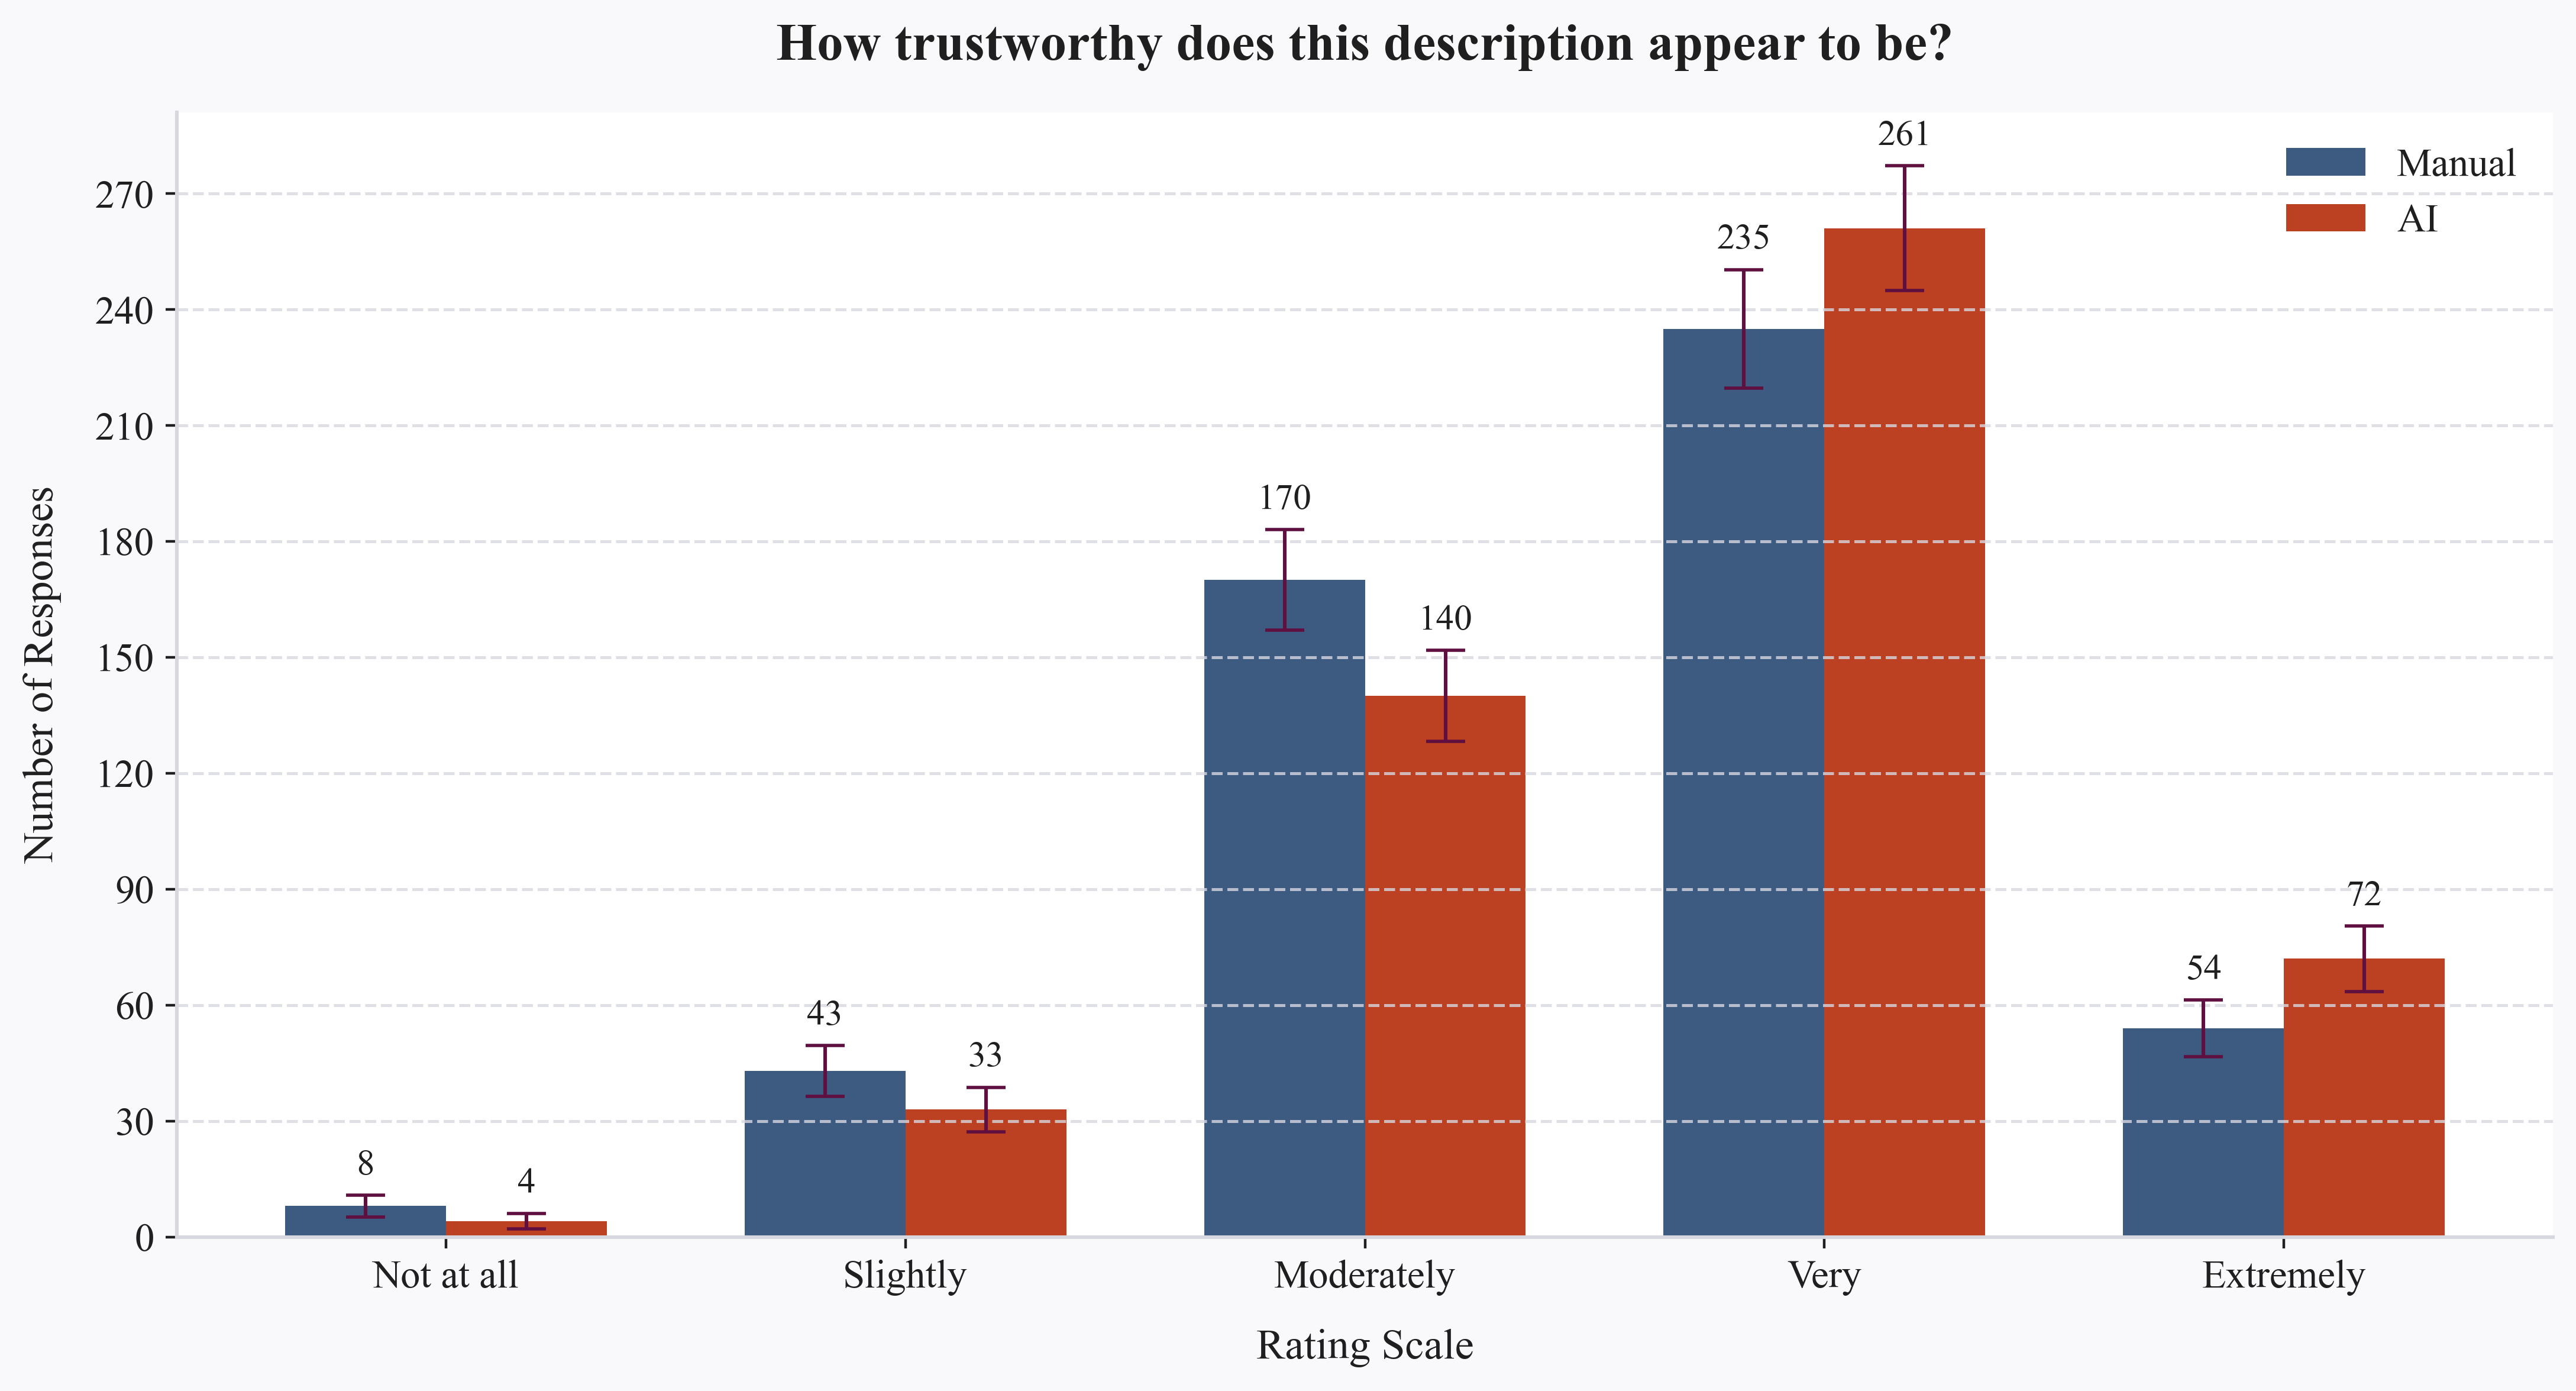
\includegraphics[width=0.85\linewidth]{figures/trust_comparison.png}
  \caption{Comparison of perceived trustworthiness between manual and AI-generated descriptions. Error bars represent Poisson-style standard error estimates computed on raw counts ($\sqrt{n}$).}
  \Description{Bar chart comparing manual and AI description ratings for trustworthiness}
  \label{fig:trust}
\end{figure}

AI-generated descriptions received higher trust ratings overall, with fewer low-trust responses and more ratings in the highest category (Extremely: 72 vs.
54). The pooled chi-square test provided borderline evidence of a distributional shift ($\chi^2(4) = 9.49$, $p = 0.050$). The effect size was small (Cramer's $V = 0.096$, computed with $N=1020$ pooled observations), indicating that the improvement is modest in magnitude and should be interpreted cautiously.

\subsection{Clarity and Completeness}
Participants evaluated how clear and complete the information was using a 5-point scale from Very Unclear to Very Clear. Figure~\ref{fig:clarity} shows the distribution of clarity ratings.

\begin{figure}[h]
  \centering
  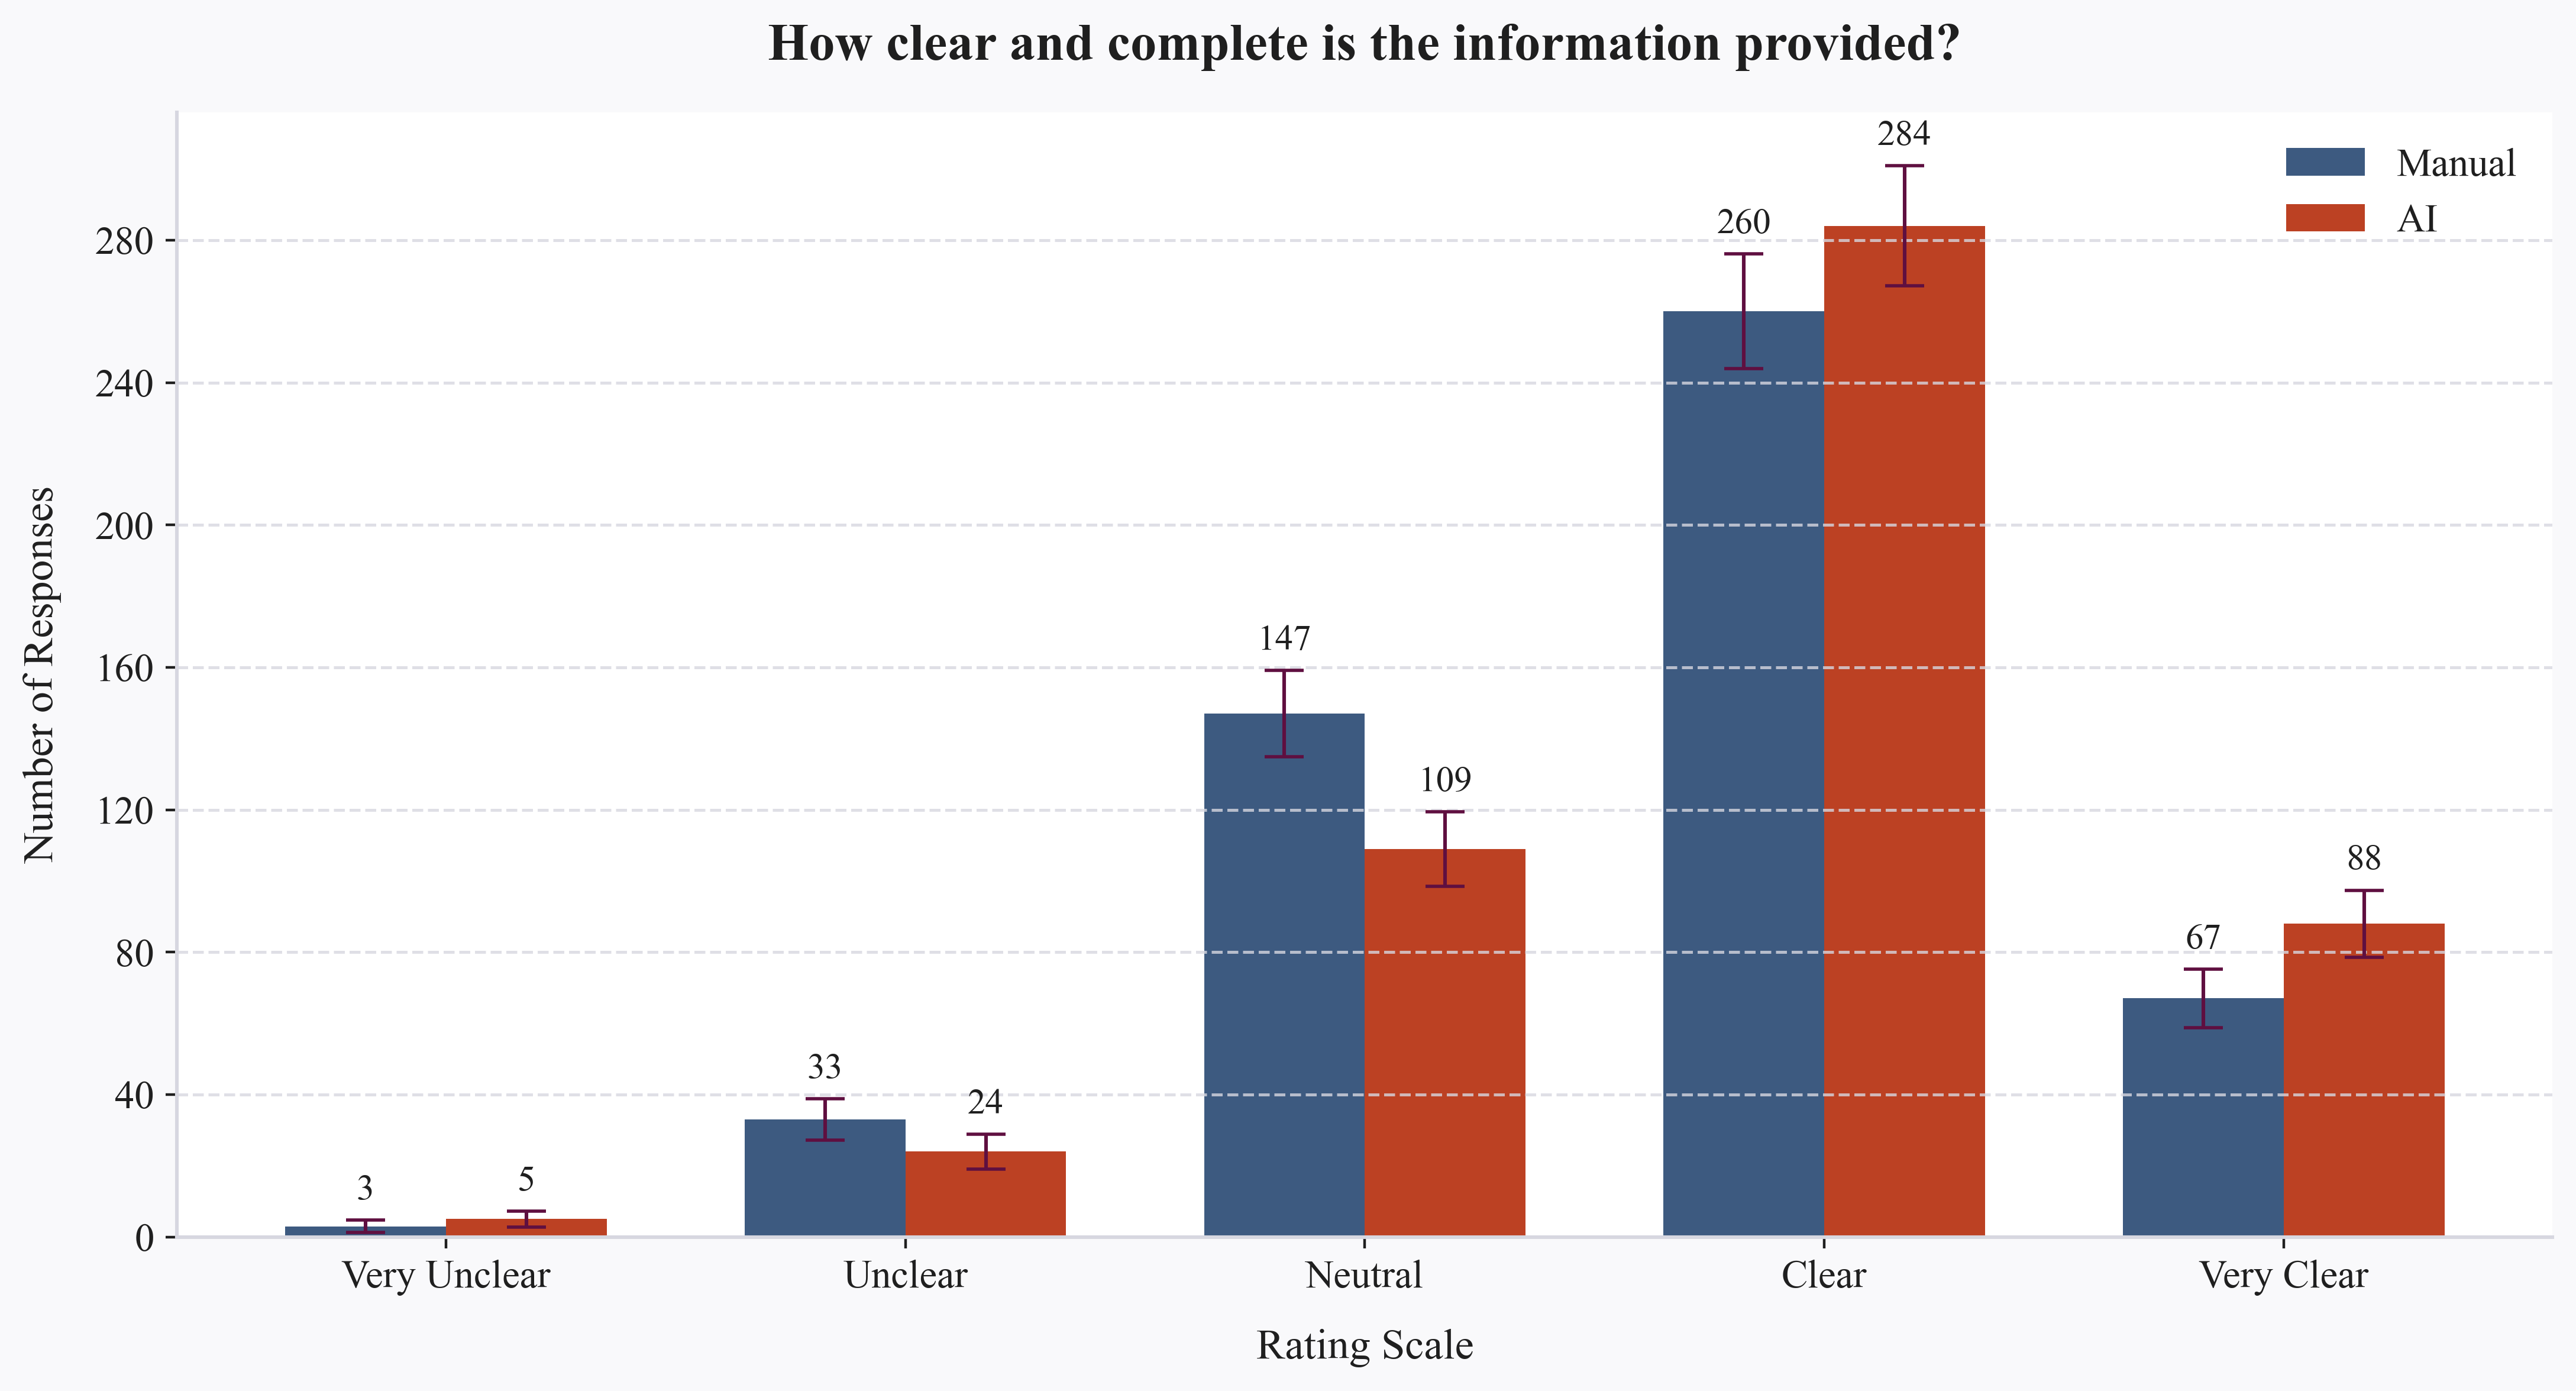
\includegraphics[width=0.85\linewidth]{figures/clarity_comparison.png}
  \caption{Comparison of perceived clarity and completeness between manual and AI-generated descriptions. Error bars represent Poisson-style standard error estimates computed on raw counts ($\sqrt{n}$).}
  \Description{Bar chart comparing manual and AI description ratings for clarity and information completeness}
  \label{fig:clarity}
\end{figure}

AI-generated descriptions were rated as clearer overall, with a notable reduction in neutral responses (109 vs.
147) and more ratings in the top two categories (Clear or Very Clear: 372 vs.
327). The pooled chi-square test indicated a statistically significant difference in the distribution ($\chi^2(4) = 11.47$, $p = 0.0218$). The effect size was small (Cramer's $V = 0.106$, computed with $N=1020$ pooled observations), consistent with a modest but systematic shift in perceived clarity.

\subsection{Comparative Preferences}
Beyond individual ratings, participants completed several comparative preference questions. Due to space constraints, this short paper reports the engaging comparison. Responses were nearly evenly split between AI-generated (221; 43.3\%) and manual (220; 43.1\%) descriptions, with 69 selections (13.5\%) indicating both versions were equally engaging. This near-parity suggests that personalization increased perceived clarity without reducing engagement.

\subsection{Overall Study Feedback}
Following the POI evaluations, participants were invited to provide optional overall feedback. A subset of 17 participants completed this section, rating three dimensions using a 5-point scale (1 = Poor, 5 = Excellent). The overall experience with POI descriptions received a mean rating of 3.88 (SD = 0.70, Median = 4.0), indicating generally positive reception. Participants expressed moderate to strong support for the concept of automatically adapting POI descriptions based on user interests, with a mean rating of 3.75 (SD = 0.93, Median = 4.0). Comfort with reading AI-generated descriptions when planning visits to new places received the highest mean rating of 3.94 (SD = 0.83, Median = 4.0), suggesting participants were receptive to AI-generated travel content when it demonstrated quality and relevance. The relatively low standard deviations (all below 1.0) indicate consensus among participants without extreme polarization of opinions.

Across metrics, AI adaptation primarily reduced neutral ratings and increased positive categories. Given the repeated-measures structure of the data, pooled tests summarize distributional shifts.
